% introduction.tex

\section{Introduction}
Voldemort is an implementation of a distributed, highly available key-value store.
The configuration of the system is however cumbersome and tedious, so we would like to explore the possibilities for using ZooKeeper to coordinate configuration and later some management tasks.
Such tasks includes extending and reducing the members of the cluster.

We have created a method for managing cluster metadata and configuration for Voldemort by using Apache ZooKeeper for coordination.

In this process we have implemented an internal StorageEngine that uses ZooKeeper for node metadata.

We have also implemented a service, named Headmaster, that manages configuration, node discovery and node membership in the cluster.
Headmaster can also decide whether to execute a rebalance based on certain criteria.

\subsection{Voldemort and Dynamo}
Voldemort is a software system based off of Amazon's paper on Dynamo, Amazons highly available key-value store.
Voldemort and Dynamo sacrifices consistency and isolation requirements to achieve higher availability with satisfactory durability.
In fact, we will later see that most of this behavior is tunable and left as design choices per implementation.


\subsection{Techniques and technologies}
The software used in this project employ many different and important techniques known from distributed computing, and will be discussed here.


\subsubsection{Durability and conflicts}

\subsubsection{PAXOS}

\subsubsection{Consistent hashing}
Consistent hashing is a technique introduced in 1997 by David Karger et al.\cite{Karger97consistenthashing}
The technique is used to solve problems with locating a key in a distributed system.
Let's assume you have $n$ servers in the system, then number these from $0$ to $n-1$.
The hashspace of the keys are then divided into $n$ partitions. Then do a $\textrm{Hash(key) mod } n$ and you have the server location for the key.

However, with this scheme if a server fails and you now have $n-1=m$ servers, all the failed server's data is gone.
You have to invalidate all existing servers, renumber your set of servers and start over.

Consistent hashing solves this problem by assigning each node with a number of points in the hash space.
The hash space is viewed as a ring by wrapping around \texttt{0000-FFFF}, and then placing nodes on several points along the ring as in Figure \ref{fig:hashring}. Here key K is routed to the next node on the ring, node B.
When a key is looked up, find it's place on the ring and move clockwise to the first assigned point.
\begin{figure}[h]
    \centering
    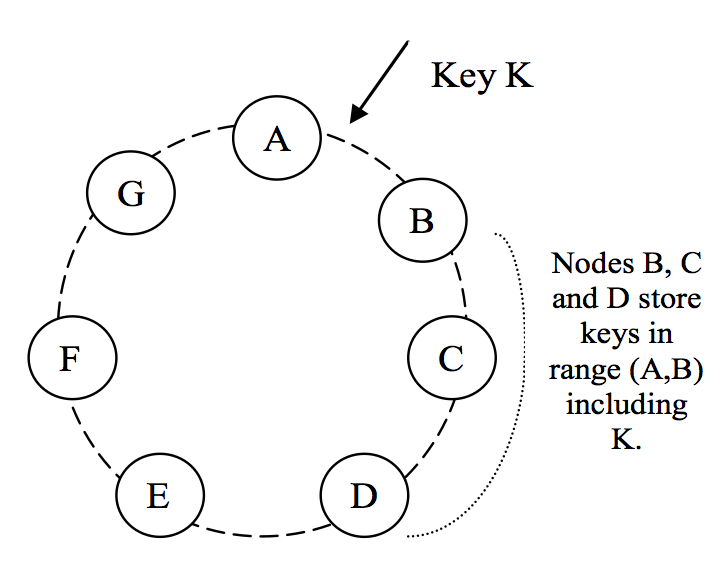
\includegraphics[width=0.5\textwidth]{introduction/hashring}
    \caption{Hash ring with several nodes. Figure from \cite{dynamo}}
    \label{fig:hashring}
\end{figure}

This approach to locating keys has several advantages:

\begin{itemize}
\item This method, like before, distributes operations on the set of available servers. By having each server take numerous positions on the hash ring, we also gain a more even distribution of the amount of keyspace among the nodes.

\item It can also accomodate different types of servers by allowing more powerful nodes to have more points assigned on the ring, and vice verca. 

\item When adding a new server, a number of different areas around the circle are affected, and not one contiguous piece. This means the work of adding in the new node will also be spread over the system, and not all requests routed to a single node.

\item The spread of the keyspace also avoids rehashing of more than $k/n$ keys when adding a new node. 

\item When a node fails, you move along the ring to the next server. If the nodes occupy several points on the ring, this means the work from a failing node is distributed among all the nodes in the system.
\end{itemize}

Consistent hashing also conveniently allows for easy, tunable replication of data to ensure durability, as used by key-value stores Dynamo\cite{dynamo} and Voldemort. Consider W the number of data replicas to create. Hash the key, then move along the ring, writing key K to the W first nodes encountered on the ring. This will also ensure backups to be available along the ring when a node fails and requests gets passed along.

\subsubsection{Membership}
gossip

\subsubsection{Failures}

\subsubsection{Tunability}
The system gives the admin the opportunity to fine tune certain parameters after what the system needs.
These are called N,R,W

\subsection{Goals}
Create a system for automatically including new nodes in a set of member nodes.
For Voldemort, this includes redistributing partitions and updating routing information without making the system unresponsive, ie. without incurring downtime.

\subsection{}

\section{Headmaster}
Headmaster is our take on managing the cluster.

It is implemented as a standalone service so that it can be run remotely, and independently from Voldemort.
We later decided to move it closer, so that we could keep better uptime on the service and reduce the chance of conflicts.
At one point we had inadvertently started two Headmasters, which kept fighting for control.
We spent a fair amount of time debugging weird race conditions until we realized there was two services listening.

It is now a master based service with leader election through ZooKeeper that can run on any number of nodes.

\section{}
